\chapter{Metodologia}
\label{cap3}

\section{Resumo}

\paragraph{} As seções a seguir trazem detalhes quanto a estrutura técnica do projeto. Portanto, a Figura \ref{fig:100} apresenta uma noção geral de como as estrutras se conectam.

\begin{figure}[h]
    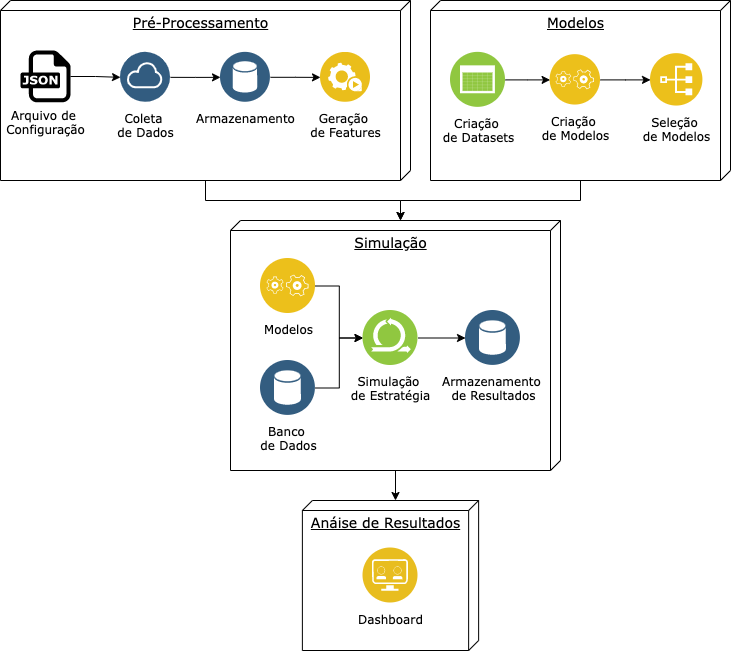
\includegraphics[scale=0.52]{resumo_projeto.png}
    \centering
    \caption{Estrutura do técnica do projeto}
    \label{fig:100}
\end{figure}

\paragraph{} Primeiro, antes da execução do código principal, é necessário garantir que os modelos estão devidamente localizados em pasta apropriada. Para isso, faz-se imprescindível a criação dos \textit{datasets} para cada ação a ser simulada, pois servem de entrada de dados para a criação e seleção dos modelos, etapa esta que deve ser executada logo em sequência. A biblioteca \textit{multiprocessing} foi utilizada para minimizar o tempo total gasto nestas etapas.

\paragraph{} Após a criação dos modelos, tem-se início a etapa de pré-processamento de dados, onde ocorre a leitura e interpretação do arquivo de configuração para se obter o número de estratégias a executar, quais os ativos envolvidos e seus recpectivos intervalos de tempo. Uma vez verificado no banco os dados já existentes, faz-se um \textit{download} apenas dos dados necessários. Se houver alguma atualização de dados, as \textit{features} de uso geral são recalculadas e armazenadas no banco a fim de servir de insumo para as estratégias que estarão por vir.

\paragraph{} Completada a etapa de pré-processamento, inicia-se a simulação das estratégias. O arquivo de configuração foi projetado para ser capaz de designar diversas estratégias de parâmetros distintos a uma mesma ordem de execução de programa. Também fez-se uso da biblioteca \textit{multiprocessing} para paralelizar as simulações, cujos resultados e estatísticas são salvas no banco para posterior análise.

\paragraph{} Por fim, é possível visualizar os resultados de forma clara através de uma aplicação secundária responsável por criar um \textit{dashboard} interativo.

\paragraph{} Em relação às tecnologias utilizadas, a aplicação foi desenvolvida em \textit{Python} com o apoio das bibliotecas \textit{yfinance}, \textit{pandas}, \textit{dash} e \textit{multiprocessing}. Foi estruturado um banco de dados \textit{PostgreSQL} para armazenamento dos \textit{candlesticks} obtidos, das \textit{features} geradas e das estratégias simuladas. Também foi incorporado o uso de \textit{Docker} especificamente para a execução de estratégias sem a necessidade de configuração de ambiente.

\section{Pré-Processamento}

\subsection{Arquivo de Configuração}
\label{sub:conf_file}

\paragraph{} O Arquivo de Configuração é um arquivo no formato JSON responsável por configurar detalhadamente cada parâmetro da sequência de estratégias que se deseja executar. Uma ordem de execução do programa pode conter diversas simulações de estratégias, que são configuradas neste Arquivo. A Figura \ref{fig:101} mostra sua estrutura.

\begin{figure}[h]
    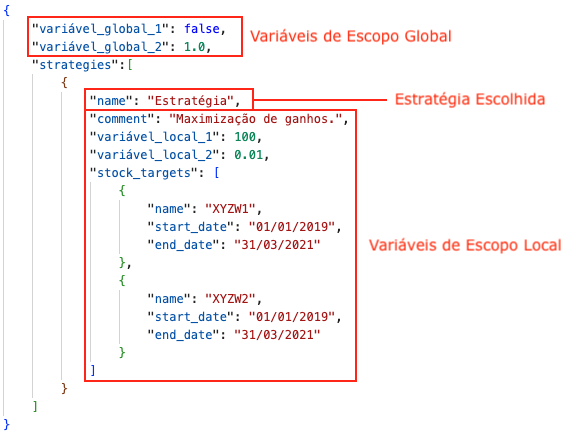
\includegraphics[scale=0.50]{config_file_estrutura.png}
    \centering
    \caption{Estrutura do Arquivo de Configuração}
    \label{fig:101}
\end{figure}

\paragraph{} Nota-se que no topo são listados os parâmetros de uso geral, ou variáveis de escopo global, de cujos valores precedem quaisquer outros listados a seguir, em caso de sobreposição. Em seguida abre-se o vetor de tipos de estratégias, onde o campo \textit{name} representa o nome da classe selecionada, sendo este o elemento que conecta o usuário ao tipo de estratégia desejada. Após a seleção do nome, são configurados os parâmetros internos da estratégia. A Tabela \ref{tab:3} da Seção \ref{sub:params_list} descreve todos os parâmetros disponíveis.

\paragraph{} Para se criar mais de um perfil de simulação, é necessário modificar o Arquivo conforme a Figura \ref{fig:102}. Automaticamente, o código interpreta que existe mais de uma simulação a executar, com todos os parâmetros em comum exceto aqueles em formato de listas. Caso haja mais de um parâmetro no formato de lista, seus comprimentos precisam ser iguais. No caso da Figura \ref{fig:102}, a primeira simulação utilizará os valores (100, 0.01) para o par (variável\_local\_1, variável\_local\_2), a segunda utilizará (200, 0.02) e assim sucessivamente.

\begin{figure}[h]
    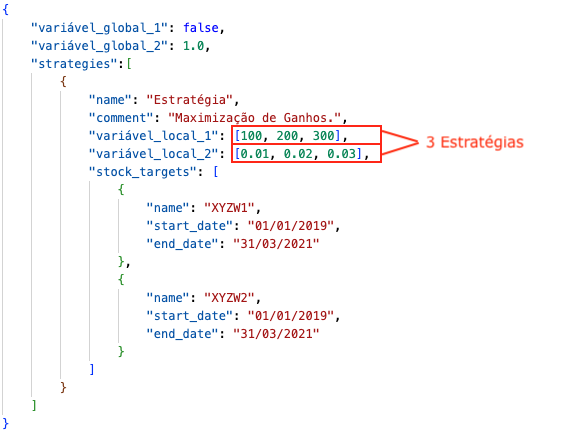
\includegraphics[scale=0.50]{config_file_mult_exec.png}
    \centering
    \caption{Arquivo de Configuração para Execuções Múltiplas}
    \label{fig:102}
\end{figure}



\subsection{Coleta de Dados}
\label{coleta_de_dados}

\paragraph{} A Coleta de Dados ocorre através da biblioteca \textit{open-source} \textit{yfinance} \cite{yfinance}, uma ferramenta não oficial que transmite dados públicos da plataforma \textit{Yahoo! Finance} \cite{yahoo_finance}, um subsistema da rede \textit{Yahoo!}.

\paragraph{} A escolha desta biblioteca como fonte primária de dados se deve principalmente pela ausência de custos associada à facilidade de uso. Contudo, alguns testes e verificações com outras fontes de dados evidenciaram destantagens significativas, porém não impeditivas para seu uso. São elas:

\begin{itemize}
    \item Os valores de proventos (i.e., dividendos e juros sobre capital próprio) que a biblioteca disponibiliza não são consistentes para a B3, portanto não são utilizados por este projeto. Testes internos confirmaram a presença de diversos proventos corretamente apresentados e ajustados pelos respectivos desdobramentos acumulados, porém somados a alguns \textit{outliers} inexistentes na realidade, o suficiente para questionar seu uso em escala (i.e., para vários ativos sem verificação individual). \color{red} HERALDO: Devo mostrar evidências do teste que corrobora esta afirmação? \colorend

    \item Os volumes de negociação disponibilizados não necessariamente coincidem com a plataforma TradingView em valores absolutos, porém coincidem em valores relativos (i.e., variação de volume dia após dia para um mesmo ativo), o que é suficiente para este trabalho. \color{red} HERALDO: (1) Na verdade, encontrei algumas evidências de que os valores relativos conferem, mas nenhum evidência de que não conferem. (2) Será que posso citar a plataforma TradingView? Ou melhor, devo tomar algum cuidado? \colorend

    \item \textit{Candlesticks} de janelas temporais inferiores à diária (\textit{intraday}) são disponibilizados, porém as limitações envolvidas inviabilizam seu uso, como: o limite de 730 dias para a busca dos dados; a inconsistência com os dados diários quanto ao volume; e a alguns \textit{bugs} como a ausência de \textit{candlesticks} em todo dia de parcial do pregão da B3 (Quarta-feira de Cinzas).
\end{itemize}

\paragraph{} Os dados obtidos são \textit{candlesticks} diários (OHLCV). Com a mesma facilidade, é possível adquirir janelas de tempo semanais, no entanto para evitar potenciais problemas de consistência de dados, as mesmas são calculadas internamente a partir da janela diária via comandos SQL\footnote{\textit{Structured Query Language}: Linguagem usada para administrar bancos de dados relacionais.}.

\paragraph{} Apenas os dados não existentes no banco são baixados via \textit{yfinance}. Para isso, um \textit{trigger}\footnote{Procedimento armazenado em um banco de dados que é chamado automaticamente sempre que ocorre um evento.} é acoplado às tabelas de \textit{candlesticks} e acionado sempre que operações de \textit{insert}, \textit{update}, \textit{delete} e \textit{truncate} são realizadas. Quando ativado, chama uma função responsável por atualizar a tabela de \textit{status}, que registra o intervalo de tempo representado nas tabelas de \textit{candlesticks} para cada \textit{ticker} envolvidos. Deve-se ressaltar que os devidos cuidados foram tomados para evitar buracos entre intervalos de tempo não adjacentes. Portanto, apenas uma consulta à tabela de \textit{status} é executada para se verificar a necessidade de \textit{download} de novos dados.



\subsection{Armazenamento de Dados}

\paragraph{} O Armazenamento de Dados é realizado por um banco de dados \textit{PostgreSQL}, criado com o objetivo de salvar: os resultados das simulações; as \textit{features} de uso geral; e os \textit{candlesticks} obtidos. As vantagens de um banco de dados em relação a um arquivo CSV ou a uma planilha de Excel dispensam comentários. Contudo, quanto ao escopo deste trabalho, pode-se mencionar os seguintes pontos:

\begin{itemize}
    \item Fácil acesso aos resultados das simulações de forma estruturada e consistente, recurso este utilizado pela aplicação que gera o \textit{dashboard} de resultados.
    \item Economia de processamento devido ao armazenamento das \textit{features} de uso geral, uma vez que estratégias simuladas não necessitam recalculá-las a cada execução.
    \item Independência da plataforma \textit{Yahoo! Finance} para o caso de não continuidade dos dados ou qualquer alteração repentida.
    \item Diminuição do tráfego na rede pela persistência dos \textit{candlesticks} já obtidos.
\end{itemize}

\paragraph{} Os \textit{candlesticks} semanais são calculados via \textit{query} SQL para garantir a consistência dos dados, já que a possibilidade de inconsistência se fez presente entre dados \textit{intraday} e diários, conforme mencionado na Seção \ref{coleta_de_dados}.

\paragraph{} A figura \ref{fig:103} mostra o ERD\footnote{\textit{Entity-Relationship Diagram}. Em português: Diagrama de Entidade Relacionamento.} do banco. Os \textit{scripts} de criação e população inicial do banco de dados pode ser encontrado em \cite{github_projeto}. \color{red} HERALDO: (1) Vale a pena mostrar o ERD do banco? (2) Devo mencionar as constraints de banco que garantem consistência, como por exemplo a comparação do preço máximo de um candle com seus outros valores a fim de garantir que este de fato é máximo? Preços não negativos, valores não nulos, etc. \colorend

\begin{figure}[h]
    
\includegraphics[scale=0.90]{no_image.jpeg}
    \centering
    \caption{ERD do Banco de Dados}
    \label{fig:103}
\end{figure}



\subsection{Geração de \textit{Features} de Uso Geral}
\label{sub:features}

\paragraph{} As \textit{Features} de Uso Geral são características derivadas dos \textit{candlesticks} que podem auxiliar qualquer decisão interna de uma estratégia, porém seu objetivo principal está no suporte à escolha do momento de entrada apropriado nas operações, o que é fundalmentalmente a responsabilidade do modelo de \textit{Machine Learning}. Como podem ser utilizadas por qualquer estratégia, são calculadas antes do início das simulações e somente quando há necessidade, ou seja, quando os \textit{candlesticks} são inseridos pela primeira vez no banco ou quando são atualizados. Ao final dos cálculos, são armazenadas nas tabelas de \textit{features} para posteriores consultas durante as simulações.

\paragraph{} Nesta etapa do projeto, assim como em diversas outras, faz-se necessário atenção e cuidados quanto a erros de não-causalidade, que mesmo sendo sutis, podem influenciar drasticamente os resultados finais. \color{red} HERALDO: Devo omitir esse parágrafo? A intenção é dizer que o autor não subestima essa problema, portanto tomou cuidados a nível de implementação para evitá-lo. Por outro lado, talvez essa preocupação já esteja subentendida, sendo desnecessário enfatizá-la. \colorend

\paragraph{} As \textit{features} de Uso Geral utilizadas são:

\begin{itemize}
    \item \sout{Média Móvel Exponencial de 17 períodos no gráfico diário.} \\
    \color{red} HERALDO: Feature original do André Moraes. Não utilizado nos modelos. \colorend

    \item \sout{Média Móvel Exponencial de 72 períodos no gráfico diário.} \\
    \color{red} HERALDO: Feature original do André Moraes. Não utilizado nos modelos. \colorend

    \item \sout{Média Móvel Exponencial de 72 períodos no gráfico semanal.} \\
    \color{red} HERALDO: Feature original do André Moraes. Não utilizado nos modelos. \colorend

    \item \sout{\textit{Flag} de Tendência de Alta.} \\
    \color{red} HERALDO: Feature original do André Moraes. Não utilizado nos modelos DA FORMA QUE O ANDRÉ USA, por isso o risco no texto. Ele se baseia em picos e vales ascendentes para justificar uma tendência de alta (de acordo com a teoria de Dow). A nível de código, a estratégia mais simples é comparar os últimos 2 picos de mínimo e 2 picos de máximo, verificar se um é maior que o outro com alguma margem de tolerância, que se caracteriza tendência de alta. Porém essa informação é ruidosa, principalmente em mercados em consolidação (=muito lateralizados). O que ocorre na prática do André, é que não são só os ultimos 4 picos que são analisados. Primeiro, ele já tira uma noção visual se o mercado anda em consolidação, isso requer olhar uma quantidade variável de picos que possuem algum grau de proximidade nas magnitudes, mas se comportam entre linhas de suporte e resistência. Quantos dias passados devo olhar para medir a consolidação? (retórica rs). Se uma ação vem em tendência de baixa, por exemplo, ele não espera exatamente o par perfeito de 4 picos ascendentes para dizer se o mercado está em alta, muitas vezes porque o quarto pico ainda nem se formou consistentemente. Tudo isso se baseia em uma boa identificação de picos, que felizmente foi implementada, porém tem um atraso mínimo de 9 dias para identificar qualquer pico. Enfim, embora possível, não é trivial uma boa métrica fidedigna ao André, seguindo esta lógica. \colorend

    \item \sout{\textit{Stop Loss} no último pico de rompimento/reversão de tendência (Pressupõe preço de compra definido).} \\
    \color{red} HERALDO: Não utilizado mais pois era feature do André Moraes. Não utilizado nos modelos. Em particular, essa não é trivial de se calcular e foi uma das quais distanciou a simulação feita da estratégia real do André. Os picos relevantes que retratam a memória do mercado muitas vezes estão relacionados a acontecimentos notáveis, como crises financeiras, acidentes industriais, relatórios jurícos, escândalos, aquisições novas, etc. O André pode não avaliar os acontecimentos menores na escolha do stop por ser grafista e não estar inteiramente ligado nas notícias, mas leva em consideração os mais marcantes. Como análise de notícias está completamente fora do escopo, obter "grau de importância" de um pico com alguma precisão requer no mínimo olhar os dados intraday (seção de coleta de dados explica porque não usei) e avaliar o volume de negociações na regiões. Contudo, idealmente deve-se olhar o livro de ofertas para tirar métricas das forças de compra e de venda, talvez aliadas ao volume de negociação e assim obter um valor razoável. Quando implementei na tentativa de simular o André, usei simplemente o pico mais próximo abaixo do preço de compra, dado uma distância mínima de 1\%. \colorend

    \item \textbf{\textit{Flag} de Identificação de Crises} \\ \\
        \textit{Flag} criado para prever crises financeiras através da identificação de anomalias nos volumes de negociação. Seu objetivo é impedir que o modelo de ML entre em qualquer operação durante sua presença. Para isso, utiliza-se a média \begin{math} \overline{V} \end{math} e o desvio padrão \begin{math} \sigma_V \end{math} do volume de negociações dos últimos 60 dias úteis, junto com o volume \begin{math} V \end{math} do dia corrente. Adiciona-se um efeito de inércia de 2 dias úteis consecutivos para ativar uma anomalia de volume e outra inércia de 8 dias úteis para persistência do \textit{flag}. As Equações \ref{eq:20} e \ref{eq:20} mostram o cálculo e a Figura \ref{fig:104} ilustra a eficácia do \textit{flag}.

        \begin{equation} \label{eq:20}
            V_{anomaly(i)} = \begin{cases} 1, & \mbox{se } V_{(i)} \ge \overline{V} + \sigma_V \quad \textrm{e} \quad V_{(i-1)} \ge \overline{V} + \sigma_V \\ 0, & \mbox{caso contr\'ario} \end{cases}
        \end{equation}

        \begin{equation} \label{eq:21}
            F_{crisis(i)} = \begin{cases} 1, & \mbox{se } V_{anomaly(i)} = 1 \\ 1, & \mbox{se } V_{anomaly(i)} = 0 \quad e \quad F_{crisis(i-1)} = 1 \quad \textrm{(At\'e 8 vezes consecutivas)} \\ 0, & \mbox{caso contr\'ario} \end{cases}
        \end{equation}

        \begin{figure}[h]
            
\includegraphics[scale=0.70]{no_image.jpeg}
            \centering
            \caption{\textit{Flag} de Identificação de Crises para a ação XYZ no período de XX/YY/ZZZZ a XX/YY/ZZZZ}
            \label{fig:104}
        \end{figure}

    \item \textbf{\textit{Flag} de Tendência de Baixa} \\ \\
    Semelhante ao \textit{Flag} de Identificação de Crises, este \textit{Flag} também tem o objetivo de impedir entrada em operações pelo modelo de ML durante sua presença. No entanto, o critério é diferente. Primeiro, calcula-se a derivada dos preços médios \begin{math} \dot{P_{mid}} \end{math} entre o dia corrente e o anterior normalizado pela média dos preços médios (Equações \ref{eq:22} e \ref{eq:23}). Em seguida, ajusta-se um filtro digital IIR passa-baixas de coeficiente de amortecimento \begin{math} \alpha \end{math} (Equação \ref{eq:24}). Por fim, acrescenta-se um efeito de inércia de 3 dias úteis consecutivos para persistência do \textit{flag} em caso de ocorrência (Equação \ref{eq:25}). \color{red} HERALDO: Devo adicionar na fundamentação um tópico falando sobre filtro digital IIR passa-baixas e mostrando de onde vem essa fórmula? \colorend

    \begin{equation} \label{eq:22}
        P_{mid} = \dfrac{P_{open} + P_{close}}{2}
    \end{equation}

    \begin{equation} \label{eq:23}
        \dot{P_{mid(i)}} = \dfrac{ P_{mid(i)} - P_{mid(i-1)} }{ \dfrac{1}{2}(P_{mid(i)} + P_{mid(i-1)}) }
    \end{equation}

    \begin{equation} \label{eq:24}
        \dot{P_{mid\_LPF(i)}} = \alpha \dot{P_{mid(i)}} + (1 - \alpha) \dot{P_{mid\_LPF(i-1)}},  \quad \textrm{onde} \quad 0 \le \alpha \le 1
    \end{equation}

    \begin{equation} \label{eq:25}
        F_{downtrend(i)} = \begin{cases} 1, & \mbox{se } \dot{P_{mid\_LPF(i)}} < 0 \\ 1, & \mbox{se } \dot{P_{mid\_LPF(i)}} \ge 0 \quad e \quad F_{downtrend(i-1)} = 1 \quad \textrm{(At\'e 3 vezes consecutivas)} \\ 0, & \mbox{caso contr\'ario} \end{cases}
    \end{equation}

    Foi utilizado \begin{math} \alpha = 0.10 \end{math}, pois trantando-se de \textit{flag} que pode impedir diretamente o fluxo de negociações, faz-se mais necessário um baixo ruído à inércia da medida. A Figura \ref{fig:109} ilustra a eficácia do \textit{flag}. \\

    \begin{figure}[h]
        
\includegraphics[scale=0.70]{no_image.jpeg}
        \centering
        \caption{\textit{Flag} de Identificação de Crises para a ação XYZ no período de XX/YY/ZZZZ a XX/YY/ZZZZ}
        \label{fig:109}
    \end{figure}

    \item \textbf{Risco Mínimo} \\ \\
    O Risco Mínimo serve de suporte à escolha do risco de entrada em uma operação, não sendo assim consumido diretamente pelo modelo de ML. Ressalta-se que o conceito de risco no escopo deste trabalho está relacionado à diferença de valor no qual o \textit{stop loss} é colocado abaixo do preço de compra (Equação \ref{eq:51}). Sua fórmula é composta por uma parcela fixa somada a uma parcela variável, conforme mostrado pela Equação \ref{eq:30}.

    \begin{equation} \label{eq:30}
        Risk_{min} = Risk_{min_f} + Risk_{min_v}
    \end{equation}

    Seja \begin{math} \Delta \end{math} a diferença entre o preço máximo e mínimo de um \textit{candlestick} (Equação \ref{eq:31}), pode-se definir \begin{math} Risk_{min_f} \end{math} como o valor mínimo de risco necessário para superar as oscilações diárias dos preços dos últimos 20 dias úteis (Equação \ref{eq:32}).

    \begin{equation} \label{eq:31}
        \Delta = P_{high} - P_{low}
    \end{equation}

    \begin{equation} \label{eq:32}
        Risk_{min_f} = \dfrac{ \sigma_{\Delta} }{ P_{mid} }
    \end{equation}

    A parcela variável \begin{math} Risk_{min_v} \end{math} representa o inverso da derivada de preços ajustada por um filtro digital IIR passa-baixas (Equações \ref{eq:24} e \ref{eq:33}), onde \begin{math} \alpha \end{math} é o coeficiente de amortecimento.

    \begin{equation} \label{eq:33}
        Risk_{min_v} = - \dot{P_{mid\_LPF(i)}}
    \end{equation}

    Diferentemente do \textit{flag} de Tendência de Baixa, foi utilizado \begin{math} \alpha = 0.30 \end{math}, uma vez que neste caso é muito mais interessante uma resposta rápida do que um baixo ruído.

    Por fim, adicionou-se um segundo filtro de passa-baixas de \begin{math} \alpha = 0.10 \end{math} apenas aos movimentos de descida dos valores de \begin{math} Risk_{min} \end{math} a fim de se aumentar a cautela apenas durante momentos mais turbulentos do mercado.

    A Figura \ref{fig:105} mostra o resultado do algoritmo para dois papéis de comportamentos distintos: MGLU3 representando um companhia com foco em alto crescimento, portanto mais instável; e ABEV3 representando uma companhia já bem consolidada no mercado, com menos oportunidades de crescimento. \color{red} HERALDO: Precisa de alguma citação aqui para suportar as afirmações feitas? \colorend \\

    \begin{figure}[h]
        
\includegraphics[scale=0.70]{no_image.jpeg}
        \centering
        \caption{Risco Mínimo para ABEV3 e MGLU3}
        \label{fig:105}
    \end{figure}

    \item \textbf{Risco Máximo} \\ \\
    O Risco Máximo serve de suporte à escolha do risco de entrada em uma operação, não sendo assim consumido diretamente pelo modelo de ML. Ressalta-se que o conceito de risco no escopo deste trabalho está relacionado à diferença de valor no qual o \textit{stop loss} é colocado abaixo do preço de compra (Equação \ref{eq:51}). A escolha do risco também implica diretamente no valor do preço alvo de uma operação, pois o mesmo é definido como 3 vezes a magnitude do risco escolhido, percentualmente acima do preço de compra.

    A ideia central está na análise estatística das subidas de preços entre os últimos picos identificados dentro do intervalo de 80 dias úteis. Portanto, primeiro se faz necessário a criação de um um algoritmo de identificação de picos, conforme mostrado pela Figura \ref{fig:106}. O método usa uma janela móvel de \begin{math} W = 17 \end{math} \textit{candles} que corre dia após dia até a data corrente e atribui votos de máximo e votos de mínimo ao maior e menor valor encontrado na janela, respectivamente. São elegíveis à picos apenas os \textit{candles} que obtiveram um mínimo de \begin{math}  floor(W / 2) = 8 \end{math} votos. Ao final, garante-se a alternância entre máximos e mínimos locais através da remoção de picos consecutivos de um mesmo tipo.

    \begin{figure}[h]
        
\includegraphics[scale=0.70]{no_image.jpeg}
        \centering
        \caption{Algoritmo de Identificação de Picos}
        \label{fig:106}
    \end{figure}

    O algoritmo implementado cumpre seu propósito pois se assemelha ao método grafista de identificação de picos \cite{moraes2007se}. O valor da janela de 17 \textit{candles} foi escolhido devido a teoria do Phi Cube \cite{moraes2007se}. \color{red} HERALDO: O estômago até embrulha quando cito essa teoria do Phi Cube, que parece mais uma tentativa desesperada de trazer algum critério a um processo caótico. Faz lembrar filme de superherói que peca por tentar justificar demais a origem de um poder com uma base científica. Talvez a teoria do ``É 17 porque dá certo'' seja tão científica quanto o Phi Cube. \colorend

    Depois da identificação de picos, extraem-se as \begin{math} n \end{math} subidas de preços de cada mínimo para o máximo consecutivo, normalizados pelo pico de mínimo (Figura \ref{fig:107} e Equação \ref{eq:40}). Em seguida, calcula-se a média \begin{math} \overline{C_{LPF(i)}} \end{math} e o desvio padrão \begin{math} \sigma_{C\_LPF(i)} \end{math} com um filtro digital IIR passa-baixas (Equações \ref{eq:41}, \ref{eq:42} e \ref{eq:43}). Finalmente, o Risco Máximo \begin{math} Risk_{max} \end{math} pode ser encontrado segundo a Equação \ref{eq:44}, onde \begin{math} G \end{math} é a constante de razão entre ganho e perda.

    \begin{figure}[h]
        
\includegraphics[scale=0.70]{no_image.jpeg}
        \centering
        \caption{Algoritmo de Identificação de Picos}
        \label{fig:107}
    \end{figure}

    \begin{equation} \label{eq:40}
        c_k = (P_{max(k)} - P_{min(k)}) / P_{min(k)}, \quad \textrm{onde } 0 < k \le n
    \end{equation}

    \begin{equation} \label{eq:41}
        \overline{C_{(i)}} = \dfrac{1}{n} \sum_{k=1}^{n} c_k
    \end{equation}

    \begin{equation} \label{eq:42}
        \overline{C_{LPF(i)}} = \alpha \overline{C_{(i)}} + (1 - \alpha) \overline{C_{LPF(i-1)}}
    \end{equation}

    \begin{equation} \label{eq:43}
        \sigma_{C\_LPF(i)} = \alpha \sigma_{C(i)} + (1 - \alpha) \sigma_{C\_LPF(i-1)}
    \end{equation}

    \begin{equation} \label{eq:44}
        Risk_{max} = \dfrac{1}{G} (\overline{C_{LPF(i)}} - 0.5\sigma_{C\_LPF(i)}), \quad \textrm{onde } G = 3
    \end{equation}

    Foi utilizado \begin{math} \alpha = 0.50 \end{math}.

    Analogamente à Figura \ref{fig:105}, a Figura \ref{fig:108} mostra o Risco Máximo para os ativos MGLU3 e ABEV3.

    \begin{figure}[h]
        
\includegraphics[scale=0.70]{no_image.jpeg}
        \centering
        \caption{Risco Máximo para ABEV3 e MGLU3}
        \label{fig:108}
    \end{figure}

\end{itemize}



\section{Simulação de Estratégia}

\subsection{Estrutura}

\paragraph{} O tema escolhido pelo presente trabalho abrange uma quantidade gigantesca de trajetos possíveis de implementação. Facilmente a imaginação mostra uma possibilidade diferente onde a intuição por detrás da pesquisa vê campo fértil para exploração. No entanto, dar vida a um projeto de engenharia envolve a delimitação de um escopo, que necessariamente restringe as possibilidades. Dessa forma, a Estrutura na qual as estratégias serão simuladas se baseia nas seguintes declarações:


\begin{itemize}
    \item Toda estratégia possui um \textbf{capital inicial}, que representa uma quantidade de capital pré-alocado para compra dos ativos financeiros. Essa quantia deve ser sempre respeitada ao longo da simulação de forma a não representar nunca um valor negativo.

    \item Toda estratégia deve possuir uma \textbf{carteira de ativos} (ou lista de ativos) com datas iniciais e finais de validade, sendo estes intervalos de tempo onde as operações podem ser realizadas. Embora se permitam intervalos diferentes, é convencionado a mesma data de início e de fim para todos os papéis.

    \item Define-se uma  \textbf{operação} como o processo de compra única de um volume de ações de um ativo seguido pela venda de todo o volume comprado, independentemente do tempo, mesmo que esta ocorra em estágios. Nota-se que apenas a venda é cabível de ocorrer em estágios (i.e., venda parcial).

    \item Toda operação possui um \textbf{preço alvo} e um \textbf{\textit{stop loss}}. O preço alvo é um valor acima do preço de compra e o \textit{stop loss} é um valor abaixo do preço de compra. Quando o mercado atinge qualquer um dos dois valores, uma venda é disparada, encerrando a operação em vigor. No entanto, considera-se uma operação de sucesso aquela que encerrou por atingir o preço alvo e uma operação de falha aquele que encerrou por atingir o \textit{stop loss}.

    \item Uma estratégia pode possuir no máximo  \textbf{uma operação em vigência} para cada \textit{ticker} em sua bolsa de ativos, portanto para que uma segunda compra ocorra no momento em que já existem papéis adquiridos, é necessários vendê-los primeiro.

    \item A \textbf{razão entre ganho e perda} predetermina a relação entre o preço alvo de venda e o \textit{stop loss} em qualquer operação. Ela indica a razão entre a diferença do preço alvo \begin{math} P_{target} \end{math} para o preço de compra \begin{math} P_{buy} \end{math} sobre a a diferença do preço de compra para o \textit{stop loss} \begin{math} P_{stop} \end{math} (Equação \ref{eq:50}). Seu valor é constante e igual a 3. \color{red} HERALDO: Devo citar o André aqui? Não achei uma referência disso no livro dele, porém tem nos vídeos. \colorend

    \begin{equation} \label{eq:50}
        G = \dfrac{P_{target} - P_{buy}}{P_{buy} - P_{stop}} = 3
    \end{equation}

    Utiliza-se o termo ``risco de uma operação" como sendo a diferença de valor no qual o \textit{stop loss} é colocado abaixo do preço de compra (Equação \ref{eq:51}).

    \begin{equation} \label{eq:51}
        Risk = \dfrac{P_{buy} - P_{stop}}{P_{buy}}
    \end{equation}

    \item Não há \textbf{operações a descoberto}.
    \item Não há \textbf{operações alavancadas}.

\end{itemize}



\subsection{Premissas}

\paragraph{} As Premissas são um conjunto de afirmações que visam complementar a Estrutura das simulações ao mesmo tempo que garantindo a integridade dos resultados, muitas vezes optando pelo pior cenário em situações inconclusivas. São elas:

\begin{itemize}
    \item O momento de decisão de \textbf{entrada em uma operação} por uma estratégia deve ocorrer está na abertura de mercado do dia corrente, mais precisamente no instante em que o preço de abertura é definido.

    \item No dia que ocorrer a compra de um ativo, não pode haver a venda do mesmo. Em outras palavras, o \textbf{período mínimo de duração de uma operação é de 2 dias úteis}.

    \item A \textbf{venda por \textit{timeout}} ocorre quando o número máximo de dias de uma operações extrapola um valor definido (ver Seção \ref{subsection:max_op_days})

    \item Devido a ausência de informações mais detalhadas que a janela de tempo diária, a seguinte ordem é priorizada durante a \textbf{venda de um ativo}:

    \begin{itemize}
        \item Venda por \textit{stop loss}
        \item Venda parcial (caso habilitada)
        \item Venda por preço alvo
        \item Venda por \textit{timeout}
    \end{itemize}

    \item Caso um \textbf{preço de venda seja pulado}, ou seja, a descontinuidade entre o preço de fechamento do dia anterior e o preço de abertura do dia corrente não englobe o valor de venda, utiliza-se o preço de abertura de mercado. A única exceção acontece para a venda por \textit{timeout}, já que se trata de uma venda compulsória que sempre ocorre no preço de fechamento do dia designado.

\end{itemize}



\subsection{Período Máximo de Dias por Operação}
\label{subsection:max_op_days}

\paragraph{} Em teoria, poderia-se permitir que operações não tivessem um período máximo de dias para serem encerradas. Contudo, isso facilmente se prova uma péssima decisão de alocação de capital em ativos que passam por uma fase de consolidação, ou seja, sem qualquer tendência. Além do ativo em questão não encerrar a operação e trazer seu lucro ou prejuízo para a carteira, o capital alocado nele não pode ser utilizado por outros ativos que eventualmente vem a lucrar. Quanto mais lucrativa tende a ser uma estratégia, maior a inércia que esta decisão pode oferecer. Portanto, optou-se por um limite finito de dias por operação.

\paragraph{} A escolha de um número adequado para o limite de dias possui alguns caminhos, resumidos entre os extremos de: um valor fixo geral; ou um valor dinâmico para cada ação. Nota-se que criar um algoritmo que escolha o valor dinâmico a partir da análise dos dados dos últimos meses para cada ação não é trivial. Assim, optou-se por um valor fixo geral, onde a base do estudo se deu na análise ações de perfis opostos.

\paragraph{} Nesta linha, um algoritmo auxiliar foi criado para varrer um período de dias passados e criar operações com diversos valores de risco, observando quais riscos levaram a operações de sucesso e quais levaram a operações de falha. Também analisou-se a distribuição de operações de sucesso de acordo com os valores de risco e o intervalo de dias corridos.

\paragraph{} De início, foi fixado um intervalo máximo de 90 dias para cada operação hipotética que o algoritmo gerou. O valor é propositalmente grande, pois sua função é apenas não forçar \textit{timeout} na maioria das operações. As Figuras \ref{fig:120} e \ref{fig:121} mostram dois histogramas dos dias das operações de sucesso que consideram o menor risco possível, isto é, o menor valor de risco que se pode utilizar a cada dia da série temporal de forma a tornar a operação de sucesso, caso exista este valor. Se não houver, é considerado operação de falha, portanto está fora dos histogramas. A legenda indica faixas onde, no caso la linha tracejada verde na Figura \ref{fig:120}, 50\% das contagens se encontram dentro dos 12 primeiros dias, e assim por diante. Foi considerado o período de 01/01/2016 a 31/12/2018.

\begin{figure}[h]
    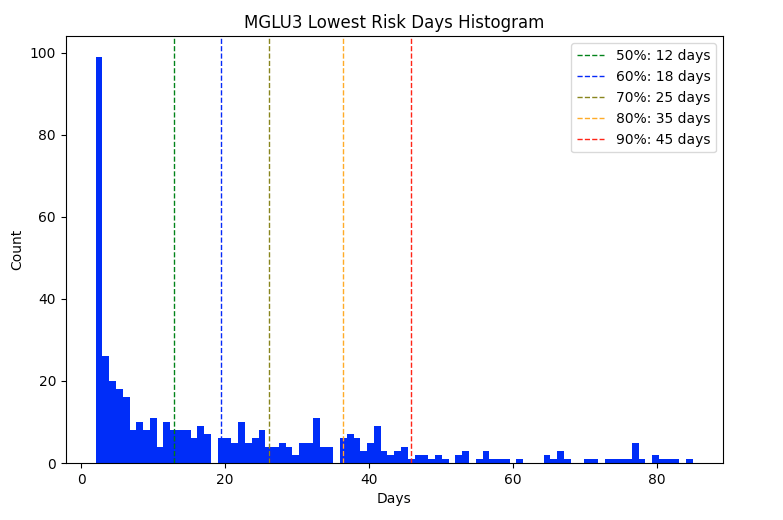
\includegraphics[scale=0.40]{MGLU3_stop_hist_min_risk.png}
    \centering
    \caption{MGLU3 - Histograma de Dias com Risco Mínimo em Operações de Sucesso}
    \label{fig:120}
\end{figure}

\begin{figure}[h]
    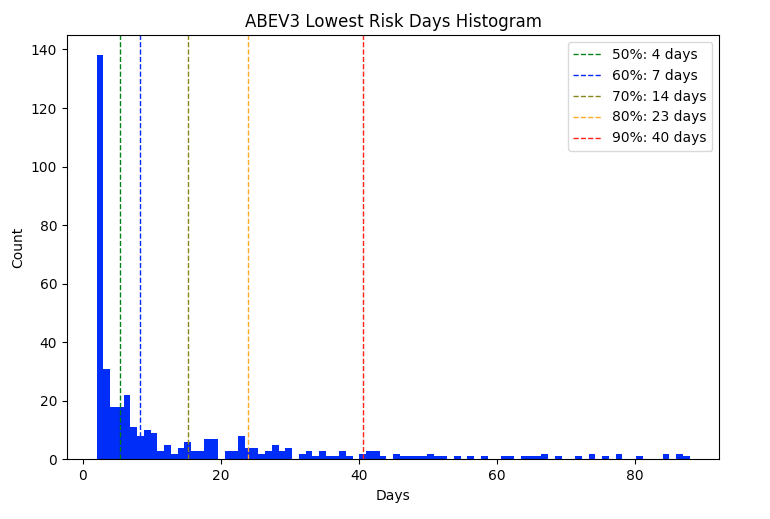
\includegraphics[scale=0.40]{ABEV3_stop_hist_min_risk.png}
    \centering
    \caption{ABEV3 - Histograma de Dias com Risco Mínimo em Operações de Sucesso}
    \label{fig:121}
\end{figure}

\paragraph{} Também foi analisado os histogramas para o caso de risco ótimo por operação, ou seja, o valor de risco que traz o maior rendimento por operação considerando os dias corridos (Figuras \ref{fig:122} e \ref{fig:123}).

\begin{figure}[h]
    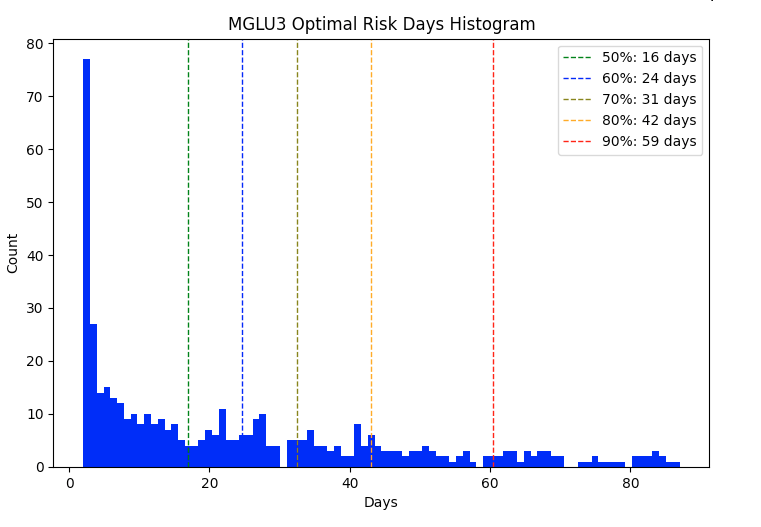
\includegraphics[scale=0.40]{MGLU3_stop_hist_opt_risk.png}
    \centering
    \caption{MGLU3 - Histograma de Dias com Risco Ótimo em Operações de Sucesso}
    \label{fig:122}
\end{figure}

\begin{figure}[h]
    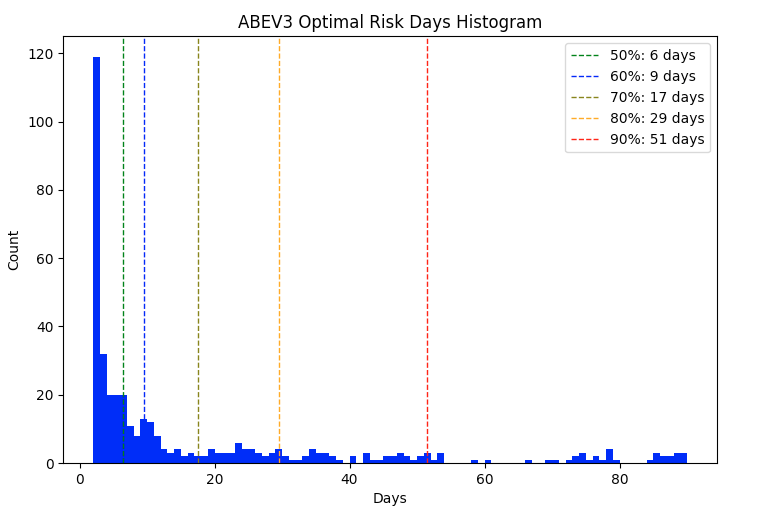
\includegraphics[scale=0.40]{ABEV3_stop_hist_opt_risk.png}
    \centering
    \caption{ABEV3 - Histograma de Dias com Risco Ótimo em Operações de Sucesso}
    \label{fig:123}
\end{figure}

A Tabela \ref{tab:4} resume o período de dias que engloba 90\% das contagens dos histogramas.

\begin{table}[h!]
    \begin{center}
        \begin{tabular}{ c|cc }
            & Menor Risco & Risco Ótimo \\
            \hline
            MGLU3 & 45 dias & 59 dias \\
            ABEV3 & 40 dias & 51 dias \\
        \end{tabular}
        \caption{Período de dias que engloba 90\% das contagens dos histogramas}
        \label{tab:4}
    \end{center}
\end{table}

\paragraph{} Com base nos valores encontrados, arbitrou-se o período máximo fixo de \textbf{45 dias} para qualquer operação. \color{red} HERALDO: É muita ousadia afirmar que escolhi arbitrariamente o valor de 45 dias com base na tabela apresentada? \colorend


\subsection{Gerenciamento de Risco}
\label{sub:risk_man}

\paragraph{} Segundo MORAES \cite{moraes2007se}, o Gerenciamento de Risco é imprescindível para um bom rendimento de uma estratégia. Afinal, não adianta obter uma alta taxa de acerto em operações de cujo lucro médio não compense as perdas acumuladas pelas operações falhadas. Além disso, estar com o capital muito alocado em ativos de um único segmento é perigoso devido à alta exposição à fatores prejudicias como falta de insumos industriais, mudanças na legislação, crises internas, instabilidade política, dentre outros.

\paragraph{} Para mitigar as questões levantadas, algumas medidas foram tomas inspiradas no trabalho de MORAES \cite{moraes2007se}. São elas:

\begin{itemize}
    \item Diversificação de ativos em segmentos de mercado variados através da escolha de um alto número de \textit{tickers}, mais especificamente 71.
    \item Criação do Coeficiente de Risco-Capital\footnote{ou \textit{Risk-Capital Coefficient} (RCC)}
\end{itemize}

\paragraph{} O Coeficiente de Risco-Capital, definido pela Equação \ref{eq:60}, é uma constante que equilibra a relação entre o capital de entrada em uma operação e o risco escolhido. Seu valor é configurado previamente no Arquivo de Configuração (ver Tabela \ref{tab:3}) e vale para todos os ativos da carteira.

\begin{equation} \label{eq:60}
    RCC = Capital \times Risk
\end{equation}

\paragraph{} Durante uma simulação, a estratégia primeiro encontra o valor do risco desejado para entrar na operação, depois escolhe o capital a ser alocado. Dessa forma, a Equação \ref{eq:61} mostra de fato a aplicação do RCC. É evidente que quanto maior o risco envolvido, menor o capital a ser alocado e vice-versa.

\begin{equation} \label{eq:61}
    Capital = \dfrac{RCC}{Risk}
\end{equation}

\paragraph{} A necessidade de um melhor uso médio de capital ao longo do período de simulação inspirou a criação de um RCC Dinâmico, que é tratado em detalhes na Seção \ref{sub:dynamic_rcc} por se tratar de uma otimização.

\paragraph{} Por fim, a Tabela \ref{tab:5} lista todos os 71 ativos escolhidos para simulação. Os critérios de escolha envolvem as seguintes preferências: diversidade de segmentos; disponibilidade da série temporal de dados a partir de 2013; e presença na composição do iBovespa em qualquer data. \color{red} HERALDO: Será que não tem outro lugar melhor para colocar essa tabela? Coloquei aqui pois foi o primeiro momento no qual foi relevante mencionar as 71 ações escolhidas, portanto aproveitei o gancho. \colorend

\begin{table}[h!]
    \begin{center}
        \begin{tabular}{ cccccccc }
            \multicolumn{8}{c}{Ações Escolhidas (71)} \\
            \hline
            ABEV3 & ALPA4 & AMER3 & B3SA3 & BBAS3 & BBDC3 & BBDC4 & BBSE3 \\
            BEEF3 & BPAN4 & BRAP4 & BRFS3 & BRKM5 & BRML3 & CCRO3 & CIEL3 \\
            CMIG4 & COGN3 & CPFE3 & CPLE6 & CSAN3 & CSNA3 & CVCB3 & CYRE3 \\
            DXCO3 & ECOR3 & EGIE3 & ELET3 & ELET6 & EMBR3 & ENBR3 & ENEV3 \\
            ENGI11 & EQTL3 & EZTC3 & FLRY3 & GGBR4 & GOAU4 & GOLL4 & HYPE3 \\
            ITSA4 & ITUB4 & JBSS3 & JHSF3 & LAME4 & LCAM3 & LREN3 & MGLU3 \\
            MRFG3 & MRVE3 & MULT3 & PETR3 & PETR4 & POSI3 & PRIO3 & QUAL3 \\
            RADL3 & RENT3 & SANB11 & SBSP3 & SULA11 & TAEE11 & TIMS3 & TOTS3 \\
            UGPA3 & USIM5 & VALE3 & VIIA3 & VIVT3 & WEGE3 & YDUQ3
        \end{tabular}
        \caption{Ações Escolhidas}
        \label{tab:5}
    \end{center}
\end{table}



\subsection{Risco de Entrada por Operação}

\paragraph{} O Risco de Entrada por Operação é encontrado a partir da média aritmética entre as \textit{features} Risco Mínimo e Risco Máximo (ver Seção \ref{sub:features}). A Equação \ref{eq:70} mostra essa relação:

\begin{equation} \label{eq:70}
    Risk_{operation} = \dfrac{1}{2}(Risk_{max} + Risk_{min}), \quad \textrm{se } Risk_{max} \ge Risk_{min}
\end{equation}

\paragraph{} Pelo fato da metodologia de cálculo do Risco Máximo e do Risco Mínimo seguirem raciocínios diferentes, podem ocorrer momentos nos quais a condição expressa na Equação \ref{eq:70} não seja verdadeira, em outras palavras, as ondas de subida de preço entre picos no gráfico diário não compensam o risco inerente ao ruído diário dos \textit{candlesticks}. Enquanto este evento ocorrer, não haverá entrada em operações para o ativo envolvido. Por outro lado, é comum uma interseção entre os períodos de Descanso por Tendência de Baixa ou até mesmo de Descanso por Identificação de Crises (Seções \ref{sub:downtrend_halt} e \ref{sub:crisis_halt}, respectivamente). \color{red} HERALDO: Algo me diz que um gráfico aqui confirmando essa interseção não seria uma má ideia, certo? \colorend



\subsection{Descanso por Tendência de Baixa}
\label{sub:downtrend_halt}

\paragraph{} O Descanso por Tendência de Baixa é um intervalo que impede qualquer nova operação durante a ativação do \textit{Flag} de Tendência de Baixa (ver Seção \ref{sub:features}). O objetivo é esperar o mercado entrar em uma nova tendência de alta ou pelo menos se estabilizar para que uma nova operação se justifique, mesmo que esta decisão implique em uma pequena inércia. Operações em vigor não são canceladas. \color{red} HERALDO: Optei por não colocar uma imagem mostrando a eficácia desse flag porque em princípio a Seção de Features (\ref{sub:features}) já faz isso. \colorend



\subsection{Descanso por Identificação de Crises}
\label{sub:crisis_halt}

\paragraph{} O Descanso por Identificação de Crises é um intervalo que impede qualquer nova operação durante a ativação do \textit{Flag} de Identificação de Crises (ver Seção \ref{sub:features}). O objetivo é esperar o mercado se estabilizar de uma crise em potencial para que uma nova operação se justifique, mesmo que esta decisão implique em uma pequena inércia. Operações em vigor não são canceladas. \color{red} HERALDO: Optei por não colocar uma imagem mostrando a eficácia desse flag porque em princípio a Seção de Features (\ref{sub:features}) já faz isso. \colorend



\subsection{Lista de Parâmetros de Configuração}
\label{sub:params_list}

\paragraph{} A Tabela \ref{tab:3} mostra uma lista de todos os parâmetros configuráveis em uma simulação. Nota-se que as variáveis de escopo geral são aplicáveis a toda e qualquer estratégia presente no Arquivo de Configuração enquanto as variáveis de escopo local dizem respeito apenas a um grupo de estratégias em parciluar (ver Seção \ref{sub:conf_file} para mais esclarecimentos).

\begin{center}
    {\small
    \begin{longtable}[m]{| m{11em} | m{3em}| m{21em} |}

        \hline
        \multicolumn{3}{|c|}{Lista de Parâmetros} \\
        \hline
        Nome do Parâmetro & Escopo & Descrição \\
        \hline
        \endfirsthead

        \hline
        \multicolumn{3}{|c|}{Continuação da Tabela \ref{tab:3}} \\
        \hline
        Nome do Parâmetro & Escopo & Descrição \\
        \hline
        \endhead

        \hline
        \endfoot

        \hline
        \multicolumn{3}{|c|}{Fim da Tabela \ref{tab:3}} \\
        \hline
        \caption{Lista de parâmetros detalhados\label{tab:3}}
        \endlastfoot

        \hline
        show\_results & Geral & Exibe \textit{dashboard} da última simulação completada ao final. Tipo: \textit{Boolean}. \textit{Default}: \textit{True}. Listável: Não. \\
        \hline
        min\_risk\_features & Geral & Risco mínimo para o cálculo de \textit{features}. Tipo: \textit{Float}. \textit{Default}: 0,01. Listável: Não. \\
        \hline
        max\_risk\_features & Geral & Risco máximo para o cálculo de \textit{features}. Tipo: \textit{Float}. \textit{Default}: 0,10. Listável: Não. \\
        \hline
        \textbf{name} & Local & \textbf{(OBRIGATÓRIO)} Nome da estratégia a ser executada. Valores válidos: ``ML Derivation". Tipo: \textit{String}. Listável: Não. \\
        \hline
        comment & Local & Comentário. Tipo: \textit{String}. \textit{Default}: \textit{String} vazia. Listável: Não. \\
        \hline
        capital & Local & Capital total da carteira em reais (R\$). Tipo: \textit{Float}. Listável: Sim. \\
        \hline
        risk\_capital\_coefficient & Local & Coeficiente de risco-capital (RCC) geral. Tipo: \textit{Float}. \textit{Default}: 0,001. Listável: Sim. \\
        \hline
        tickers\_bag & Local & Grupo de ativos a escolher dentro de ``stock\_targets". Valores aceitos: ``listed\_first" (ordem de listagem); ``random" (ordem aleatória). \textit{Default}: ``listed\_first". Listável: Sim. \\
        \hline
        tickers\_number & Local & Número de ativos a escolher dentro de ``stock\_targets", de acordo com ``tickers\_bag". Tipo: \textit{Int}. \textit{Default}: 0 (todos). Listável: Sim. \\
        \hline
        min\_order\_volume & Local & Volume mínimo por operação. Tipo: \textit{Int}. \textit{Default}: 1. Listável: Sim. \\
        \hline
        gain\_loss\_ratio & Local & Razão entre ganho e perda. Para uma unidade de risco (delta pencentual entre preço de compra e \textit{stop loss}) são utilizadas N unidades de risco acima no preço preço de compra para definir o preço alvo. Tipo: \textit{Float}. \textit{Default}: 3. Listável: Sim. \\
        \hline
        max\_days\_per\_operation & Local & Número máximo de dias por operação. Inclui o dia de compra. Caso excedido, ocorre venda compulsória pelo preço de fechamento no último dia da contagem. Tipo: \textit{Int}. \textit{Default}: 45. Listável: Não. \\
        \hline
        min\_risk & Local & Risco mínimo por operação. Tipo: \textit{Float}. \textit{Default}: 0,003. Listável: Sim. \\
        \hline
        max\_risk & Local & Risco máximo por operação. Tipo: \textit{Float}. \textit{Default}: 0,10. Listável: Sim. \\
        \hline
        max\_risk & Local & Risco máximo por operação. Tipo: \textit{Float}. \textit{Default}: 0,10. Listável: Sim. \\
        \hline
        enable\_frequency\hspace{2em} \_normalization & Local & Uso de normalização por frequência de operações. Ativos com N vezes mais operações que a média receberão N vezes menos capital. Ver Seção \ref{freq_norm}. Tipo: \textit{Boolean}. \textit{Default}: \textit{False}. Listável: Sim. \\
        \hline
        enable\_profit\hspace{4em} \_compensation & Local & Uso de compensação por lucratividade acumulada. Ver Seção \ref{profit_comp}. Tipo: \textit{Boolean}. \textit{Default}: \textit{False}. Listável: Sim. \\
        \hline
        enable\_crisis\_halt & Local & Bloqueio de novas aquisições em caso de identificação de potenciais crises financeiras (para ativo). Ver Seção \ref{sub:crisis_halt}. Tipo: \textit{Boolean}. \textit{Default}: \textit{False}. Listável: Sim. \\
        \hline
        enable\_downtrend\_halt & Local & Bloqueio de novas aquisições em caso de identificação de tendências de baixo nos preços (para ativo). Ver Seção \ref{sub:downtrend_halt}. Tipo: \textit{Boolean}. \textit{Default}: \textit{False}. Listável: Sim. \\
        \hline
        enable\_dynamic\_rcc & Local & Uso de Coeficiente de Risco-Capital dinâmico (para carteira). Ver Seção \ref{sub:dynamic_rcc}. Tipo: \textit{Boolean}. \textit{Default}: \textit{False}. Listável: Sim. \\
        \hline
        dynamic\_rcc\_reference & Local & Valor de referência de uso de capital médio no controle do RCC dinâmico. Ver Seção \ref{sub:dynamic_rcc}. Tipo: \textit{Float}. \textit{Default}: 0,80. Listável: Sim. \\
        \hline
        dynamic\_rcc\_k & Local & Valor do ganho proporcional K no controle do RCC dinâmico. Ver Seção \ref{sub:dynamic_rcc}. Tipo: \textit{Float}. \textit{Default}: 3. Listável: Sim. \\
        \hline

        purchase\_margin & Local & Margem percentual aplicada ao valor de compra. Ex: Se o alvo de compra estiver configurado para R\$100, uma margem de 1\% permitirá a compra antecipada em R\$99. Tipo: \textit{Float}. \textit{Default}: 0. Listável: Sim. \\
        \hline
        stop\_margin & Local & Margem percentual aplicada ao valor do \textit{stop loss}. Ex: Se o \textit{stop} estiver configurado para R\$100, uma margem de 1\% permitirá a compra antecipada em R\$101. Tipo: \textit{Float}. \textit{Default}: 0. Listável: Sim. \\
        \hline
        partial\_sale & Local & Uso de saídas parciais. Tipo: \textit{Boolean}. \textit{Default}: \textit{False}. Listável: Sim. \\
        \hline
        stop\_type & Local & Tipo de \textit{stop loss} utilizado. Valores aceitos: ``normal"; ``staircase" (para cada patamar de unidade de risco que o preço atinge acima do valor de compra, o \textit{stop} sobe igualmente, até uma unidade de risco abaixo do preço alvo). Ver ``gain\_loss\_ratio". \textit{Default}: ``normal". Listável: Sim. \\
        \hline
        min\_days\_after\_successful \_operation & Local & Mínimo de dias sem novas aquisições após operação de sucesso, para cada ação. Ex: para 1 dia mínimo, se a última venda de sucesso ocorreu durante o dia X, a próxima compra só ocorrerá a partir do dia X+2, inclusive. Tipo: \textit{Int}. \textit{Default}: 0. Listável: Sim. \\
        \hline
        min\_days\_after\_failure \_operation & Local & Mínimo de dias sem novas aquisições após operação de falha, para cada ação. Ex: para 1 dia mínimo, se a última venda de falha ocorreu durante o dia X, a próxima compra só ocorrerá a partir do dia X+2, inclusive. Tipo: \textit{Int}. \textit{Default}: 0. Listável: Sim. \\
        \hline

        \textbf{stock\_targets} & Local & \textbf{(OBRIGATÓRIO)} \textit{Array} de ações a incluir na carteira. Formato indicado pela Figura \ref{fig:101}. Atenção ao parâmetro ``tickers\_bag". \\
        \hline

    \end{longtable}}
\end{center}



\subsection{Ensaios Paralelos}

\color{red} HERALDO: Vou fazer apenas uma introdução para te mostrar o caminho que seguirei caso você julgue que valha a pena mencionar essa seção. Se não for necessário, removo as referências dos parâmentros mencionados ao longo desta monografia.\colorend

\paragraph{} Alguns parâmetros não se mostraram eficazes em melhorar a performance das simulações, muito embora tenham se apresentado como alternativas plausíveis na resolução de problemas ao longo deste trabalho. São eles os parâmetros:

\begin{itemize}
    \item Venda Parcial (partial\_sale)
    \color{red} HERALDO: A motivação da criação desse parâmetro vem de uma prática do André como uma forma de auxiliar o fator psicológico do trader para os casos frustantes em que o mercado quase chega no preço de venda, mas depois cai e bate no stop. Ele não usa isso constantemente, mas deixa como uma opção. Venda parcial em uma operação é vender 50\% do volume de compra adquirido quando o preço bater uma unidade de risco (1un Risco = Pcompra - StopLoss) acima do preço de compra. Dessa forma, ao invés da operação ter um ganho de 3X para cada X de possível perda, ela teria um ganho de 2X para os mesmos X, mais os casos de saída sem prejuízo. A grande questão é que essa conta não compensa, seja quando eu estava tentando replicar a estratégia do André, seja com os modelos de ML agora, nunca trouxe um rendimento maior. \colorend

    \item Saídas Parcias (stop\_type = ``staircase")
    \color{red} HERALDO: É uma extensão que criei derivada da Venda Parcial para tentar granularizar um pouco mais o critério anterior e verificar se o problema da ineficácia estava na escolha do limiar de venda. Igualmente não traz melhora alguma. A ideia é: cada vez que o preço de marcado toca o limiar de uma unidade de risco (1un Risco = Pcompra - StopLoss) acima do preço de compra, o stop loss sobre igualmente 1 un de risco. Exemplo: se o preço de compra é Pcom e o Stop Loss é Pcom - X, quando o preço de mercado atingir Pcom + X, o Stop Loss sobe para Pcom. Quando subir de novo para Pcom + 2X, o Stop sobe para Pcom + X. O alvo continua sendo Pcom + 3X como sempre. \colorend

    \item Dias Mínimos de Espera após Operação de Falha (min\_days\_after\_failure\_operation)
    \item Dias Mínimos de Espera após Operação de Sucesso (min\_days\_after\_successful\_operation)
    \color{red} HERALDO: A motivação de ambos os parâmetros aqui era diminuir o ruído de entrada e saída em operações sequenciais que o modelo de ML arrisca, mas toda hora a operação é stopada. São regiões do gráfico que apresentam 2, 3, 4 operações de falha curtas e seguidas, eventualmente com uma de sucesso e já volta pra falha. Na minha interpretação, os motivos da existência dessas regiões tem a ver com a qualidade do modelo, porém mais especificamente com: (1) a semelhança forte do momento presente com um passado de treinamento onde houve muito sucesso, muito embora possa ser apenas coincidência; e (2) a escolha de um valor de risco de entrada muito baixo para a volatilidade atual do mercado, porém sufiente para o modelo arriscar a operação (pode se somar aqui o efeito indicado em (1)). Moral da história: algumas vezes funcionou (com modelos anteriores que já discartei), porém mesmo QUANDO funciona, é difícil ter clareza do número ótimo de dias para ambos os parâmetros. Digo isso pois acontece do valor de dias escolhido estar em uma região da curva instável onde a melhora do rendimento geral foi coincidência. A prova disso se dá quando você escolhe valores imediatamente próximos e verifica novos resultados discrepantes (simulando sempre com os 71 tickers em uma carteira de 100000 reais). Enfim, eles estão sempre aqui como opções, mas são são consistentes. \colorend


\end{itemize}



\section{Otimizações de Gerenciamento de Carteira}

\subsection{Resumo}

\paragraph{} As otimizações apresentadas nesta Seção independem de um modelo de ML específico, sendo portanto algoritmos gerais que, motivados ou não por problemas oriundos dos modelos, buscam uma abordagem geral para aumento da performance da carteira.

\subsection{Normalização por Frequência de Operações}
\label{freq_norm}
\paragraph{} Cada ativo de uma carteira possui um critério próprio de análise das condições de mercado que o auxilia na decisão de entrada nas operações. Muitas vezes, ativos diferentes acumulam um número bastante variado de operações concluídas ao longo da simulação. Por outro lado, esse número não posui ligação direta com a performance individual dos mesmos. Em outras palavras, facilmente ocorre a situação de um \textit{ticker} monopolizar grande parte do capital total da carteira ao longo do tempo, simplesmente por ter uma frequência de operações maior que os outros, sem qualquer fator meritocrático que embase uma justificativa.

\paragraph{} A fim de se endereçar essa questão, foi criado o critério de Normalização por Frequência de Operações, onde cada ativo receberá de capital para uma determinada operação um valor inversamente proporcional a frequência de operações acumulada até o momento.

\begin{equation} \label{eq:80}
    Capital_{norm} = Capital \times \dfrac{ \overline{f_{total}} }{ f_{stock}}
\end{equation}

\begin{equation} \label{eq:81}
    \overline{f_{total}} = \dfrac{ N_{total\_operations} }{ N_{total\_stocks} }
\end{equation}

\paragraph{} As Equações \ref{eq:80} e \ref{eq:81} mostram a obtenção do novo Capital Normalizado \begin{math} Capital_{norm} \end{math} a partir do capital que em princípio seria alocado (ver Equação \ref{eq:61}), a frequência média de operações totais acumulada \begin{math} \overline{f_{total}} \end{math} e a frequência média de operações do ativo envolvido \begin{math} f_{stock} \end{math}, igualmente acumulada.

\paragraph{} Para a Normalização começar a ser aplicada a um ativo, é necessário que haja pelo menos uma operação concluída do mesmo, assim como um mínimo de duas vezes o número total de ativos na carteira em operações concluídas. A Equação \ref{eq:82} mostra as condições citadas.

\begin{equation} \label{eq:82}
    f_{stock} > 0, \quad N_{total\_operations} \ge 2 \times N_{total\_stocks}
\end{equation}

\paragraph{} As Figuras \ref{fig:130} e \ref{fig:131} mostram eficácia do critério criado para a simulação dos 71 \textit{tickers} listados na Tabela \ref{tab:5}, durante o período de 01/01/2019 a 31/12/2021, onde a Figura \ref{fig:130} desabilita a Normalização e a Figura \ref{fig:131} habilita.

\begin{figure}[h]
    
\includegraphics[scale=0.70]{no_image.jpeg}
    \centering
    \caption{Simulação sem uso da Normalização por Frequência de Operações}
    \label{fig:130}
\end{figure}

\begin{figure}[h]
    
\includegraphics[scale=0.70]{no_image.jpeg}
    \centering
    \caption{Simulação com uso da Normalização por Frequência de Operações}
    \label{fig:131}
\end{figure}

\paragraph{} A Tabela \ref{tab:6} traz um comparativo dos resultados das simulações. Observa-se que o critério de Normalização criado se auto-compensa, ou seja, realoca capital dentro da própria estratégia sem alterar o Uso Médio de Capital da carteira. A vantagem de um critério auto-compensado é que ele não traz uma potencial ilusão de melhora de performance, já que a comparação de resultados entre estratégias precisa ter em vista Usos Médios de Capital razoavelmente próximos entre si para que a escolha dos RCCs individuais não influencie a análise.

\begin{table}[h!]
    \begin{center}
        \begin{tabular}{ c|cc }
            & hue & hue \\
            \hline
            hue & hue & hue \\
            hue & hue & hue \\
        \end{tabular}
        \caption{Comparação de Resultados}
        \label{tab:6}
    \end{center}
\end{table}

\paragraph{} (Mencionar mais comentários sobre os outros parâmetros quando tiver as imagens e a tabela).



\subsection{Compensação por Lucratividade}
\label{profit_comp}

\paragraph{} A Compensacão por Lucratividade é um ajuste auto-compensado\footnote{Realoca capital dentro da própria estratégia sem alterar o Uso Médio de Capital da carteira} que aumenta o capital em operações de \textit{tickers} que possuem um lucro acumulado acima da média da carteira. Da mesma forma, também diminui o capital daqueles que estão com o lucro acumulado abaixo da média da carteira.

\paragraph{} A Equação \ref{eq:90} mostra a primeira etapa do cálculo da Compensação, onde \begin{math} \sigma_{eq} \end{math} é o valor em unidades de desvio padrão do quanto o lucro acumulado \begin{math} p_t \end{math} do ativo está em relação à média \begin{math} \overline{P_w} \end{math} e desvio padrão \begin{math} \sigma_w \end{math} da carteira.

\begin{equation} \label{eq:90}
    \sigma_{eq} = \dfrac{p_t - \overline{P_w}}{\sigma_w}
\end{equation}

\paragraph{} Em seguida, a Equações \ref{eq:91} e \ref{eq:92} dão sequência ao cálculo criando as constantes que serão utilizadas diretamente na Compensação. Nota-se que \begin{math} C_{max} \end{math} é a variação máxima positiva que a Compensação pode alcançar. \begin{math} \sigma_s \end{math} e \begin{math} \sigma_e \end{math} são limiares de \begin{math} \sigma_{eq} \end{math} que definem lugares geométricos diferentes.

\begin{equation} \label{eq:91}
    m_1 = \dfrac{ C_{max} }{ \sigma_e - \sigma_s }, \quad n_1 = 1 - \sigma_s m_1
\end{equation}

\begin{equation} \label{eq:92}
    m_2 = \dfrac{ C_{max} }{ \sigma_e - \sigma_s }, \quad n_2 = 1 + \sigma_s m_2
\end{equation}

\paragraph{} Finalmente, a Equação \ref{eq:93} mostra o cálculo final, que pode ser facilmente visualizado pela Figura \ref{fig:140}.

\begin{equation} \label{eq:93}
    C = \begin{cases} m_1 \sigma_{eq} + n_1, & \mbox{se } \sigma_{eq} \ge \sigma_s \quad \textrm{e} \quad \sigma_{eq} \le \sigma_e \\ m_2 \sigma_{eq} + n_2, & \mbox{se } \sigma_{eq} \le - \sigma_s \quad \textrm{e} \quad \sigma_{eq} \ge - \sigma_e \\ 1 + C_{max}, & \mbox{se } \sigma_{eq} > \sigma_e \\ 1 - C_{max}, & \mbox{se } \sigma_{eq} < - \sigma_e \\ 0, & \mbox{se } |\sigma{eq}| < \sigma_s \end{cases}
\end{equation}

\pgfmathsetmacro{\cmax}{0.6}
\pgfmathsetmacro{\sigs}{0.2}
\pgfmathsetmacro{\sige}{2.0}

\begin{figure}[h]
    \centering
    \begin{center}
        \begin{tikzpicture}
            \begin{axis}
            [
                ylabel={Compensa\c{c}\~ao [-]},
                xlabel={$Lucro [\sigma_{eq}]$},
                xmin=-3, xmax=3,
                ymin=0, ymax=2,
                xtick={-3, -2, -1, 0, 1, 2, 3},
                ytick={0, 0.2, 0.4, 0.6, 0.8, 1, 1.2, 1.4, 1.6, 1.8, 2.0},
                ymajorgrids=true,
                xmajorgrids=true,
                grid style=dashed,
            ]
            \addplot[line width=0.50mm, domain=-\sigs:\sigs,blue]{1};
            \addplot[line width=0.50mm, domain=\sigs:\sige,blue]{x * \cmax / (\sige - \sigs) + (1 - \cmax * \sigs / (\sige - \sigs))};
            \addplot[line width=0.50mm, domain=-\sige:-\sigs,blue]{x * \cmax / (\sige - \sigs) + (1 + \cmax * \sigs / (\sige - \sigs))};
            \addplot[line width=0.50mm, domain=\sige:10,blue]{1 + \cmax};
            \addplot[line width=0.50mm, domain=-10:-\sige,blue]{1 - \cmax};
            \end{axis}

        \end{tikzpicture}
    \end{center}
    \caption{Gráfico da Função de Compensação por Lucratividade}
    \label{fig:140}
\end{figure}

\paragraph{} Utilizou-se \begin{math} C_{max} = 0.60\end{math}, \begin{math} \sigma_s = 0.2 \end{math} e \begin{math} \sigma_e = 2.0 \end{math}.

\paragraph{} A Figura \ref{fig:141} mostra o ganho de performance obtido para a simulação dos 71 \textit{tickers} listados na Tabela \ref{tab:5}, durante o período de 01/01/2019 a 31/12/2021. Ressalta-se que nenhuma outra Otimização de Gerenciamento de Carteira foi utilizada a fim de se isolar o efeito desta Compensação.

\begin{figure}[h]
    
\includegraphics[scale=0.70]{no_image.jpeg}
    \centering
    \caption{Ganho de performance pelo uso da Compensação por Lucratividade}
    \label{fig:141}
\end{figure}

\paragraph{} A Figura \ref{fig:142} também mostra o ganho de performance nas mesmas condições da Figura \ref{fig:141}, com a exceção do uso comum da Normalização por Frequência de Operações, o que mostra que ambas as otimizações de carteira não se exluem, muito pelo contrário.

\begin{figure}[h]
    
\includegraphics[scale=0.70]{no_image.jpeg}
    \centering
    \caption{Ganho de performance pelo uso da Compensação por Lucratividade (com NFO)}
    \label{fig:142}
\end{figure}



\subsection{Controle Proporcional para Uso de Capital (Risco Dinâmico)}
\label{sub:dynamic_rcc}

% \paragraph{} A criação de um RCC como ferramenta de gerenciamento de risco (ver Seção \ref{sub:risk_man}) não resolve o problema de subaproveitamento do Uso de Capital da carteira ao longo do período de simulação. Entende-se por subaproveitamento a parcela de capital ocioso que, por não estar empregado em nenhum ativo, resulta em uma perda de performance geral.

\paragraph{} A criação de um RCC fixo pode ser interessante do ponto de vista de Gerenciamento de Risco (ver Seção \ref{sub:risk_man}), mas na prática deixa um pouco a desejar por requerer uma noção prévia de um valor adequado. Esse valor só pode ser obtido através de simulações anteriores ao período desejado, onde o comportamento do mercado pode ser suficientemente diferente a ponto de requerer um novo RCC, dificultando um bom ajuste. Em outras palavras, um RCC fixo leva a problemas de subaproveitamento do Uso de Capital da carteira.

\paragraph{} A solução desse problema se dá pela criação de um RCC Dinâmico, configurado através de um Controle Proporcional. A vantagem dessa abordagem está na diminuição da sensibilidade do RCC em relação à performance geral, permitindo um ajuste menos preciso sem grande impacto de performance. Tudo isso aliado a um rebalanceamento dinâmico de capital em função do uso médio de capital vigente, ou seja, períodos com menores oportunidades de operações terão mais disponibilidade de capital e vice-versa.

% \paragraph{} \color{red} HERALDO: Pensei em colocar um diagrama desse controle proporcional aqui, porém o bloco que representaria a planta (i.e., estratégia) é extremamente não-linear. \colorend

\paragraph{} As Equações \ref{eq:100} e \ref{eq:101} mostram o cálculo do RCC dinâmico (\begin{math} RCC_{din} \end{math}) a partir do RCC fixo (\begin{math} RCC_{fix} \end{math}, definido pela Equação \ref{eq:60}), do valor de referência para o uso médio de capital (\begin{math} C_{ref} \end{math}), da constante de ganho proporcional (\begin{math} K \end{math}) e do uso médio de capital dos últimos 10 dias de simulação (\begin{math} \overline{C_{10d}} \end{math}).

\begin{equation} \label{eq:100}
    e = C_{ref} - \overline{C_{10d}}, \quad \mbox{para } 0 \le C_{ref}, \overline{C_{10d}} \le 1
\end{equation}

\begin{equation} \label{eq:101}
    RCC_{din} = RCC_{fix} (1 + K e)
\end{equation}

\paragraph{} Foi utilizado \begin{math} C_{ref} = 1.0 \end{math}, \begin{math} K = 5 \end{math} e \begin{math} RCC_{fix} = 0.003 \end{math}

\paragraph{} A Figura \ref{fig:150} mostra o ganho de performance obtido pela implementação do RCC Dinâmico com os valores mencionados.

\begin{figure}[h]
    
\includegraphics[scale=0.70]{no_image.jpeg}
    \centering
    \caption{Ganho de performance pelo uso do RCC Dinâmico}
    \label{fig:150}
\end{figure}

\paragraph{} (Falar que essa medida aumenta o uso de capital mal alocado, mas aumenta ainda mais o bem alocado, por isso tem um limite)

\paragraph{} (Mostrar que RCC dinâmico não tem problema com otimizações anteriores)

% \paragraph{} A dificuldade em se distinguir um capital bem alocado de um capital subaproveitado é inerente à imperfeição do modelo escolhido. Contudo, medidas podem ser tomadas para

% Em outras palavras, idealmente se deseja que todo capital esteja alocado em algum ativo em tendência de alta para se maximizar a performance geral, no entanto isso raramente ocorre.

% \paragraph{} O primeiro e mais simples motivo é porque nem sempre todos os ativos estão em uma tendência de alta aos olhos do que qualquer estratégia possa identificar, pois nenhum algoritmo é perfeito. Assim, independentemente da realidade, existirão momentos nos quais nenhum ativo da carteira se mostra vantajoso o suficiente para existir alguma operação.


% \begin{math} R_b \end{math}
% \color{red} HERALDO: \colorend



\section{Criação de Modelos}

\subsection{Resumo}
\paragraph{}

\subsection{\textit{Baseline}}
\label{sub:baseline}
\paragraph{}

\subsection{\textit{Walk Forward Optimization}}
\paragraph{}

\subsection{\textit{Feature Selection}}
\paragraph{}

\subsection{Geração de \textit{Datasets}}
\paragraph{}

\subsection{Critérios de Escolha}
\paragraph{}


\section{Análise de Resultados}
\paragraph{} EXCLUIR - Dashboard; Baseline